This chapter presents the findings of the study and engage in a detailed analysis of the results. 

\section{Training YOLO}
The training was performed following the steps presented in Ultralytics documentation \cite{YOLOTraining}. To achieve higher performance, the algorithm was implemented in Google Colaboratory. Google Colaboratory is a web-based application for creating and sharing computational documents with code, data, and output, while also allowing access to specific GPUs.

\subsection{Dataset}
The VisDrone2019 dataset consists of 288 video clips formed by 261,908 frames and 10,209 static images, captured by various drone-mounted cameras, covering a wide range of aspects including location (taken from 14 different cities separated by thousands of kilometers in China), environment (urban and country), objects (pedestrian, vehicles, bicycles, etc.), and density \cite{VisDrone}. VisDrone comes with a set of text files (one for each image), but the annotation format must be converted to YOLO format in order to allow the training process. 

\subsection{Evaluation of Results}
As stated in \citen{lin2015microsoftcococommonobjects}, evaluating results on multi-class datasets is challenging due to the presence of multiple class instances per image, the non-uniform class distribution that makes simple accuracy measures inadequate, and the need for algorithm-independent evaluation measures. Mean Average Precision was used to evaluate both classification and detection in VOC2007 \cite{PascalVOC}. The mAP evolution during training for our system is shown in Figure \ref{mAPssistema}.

\begin{figure}[h]
	\centering
	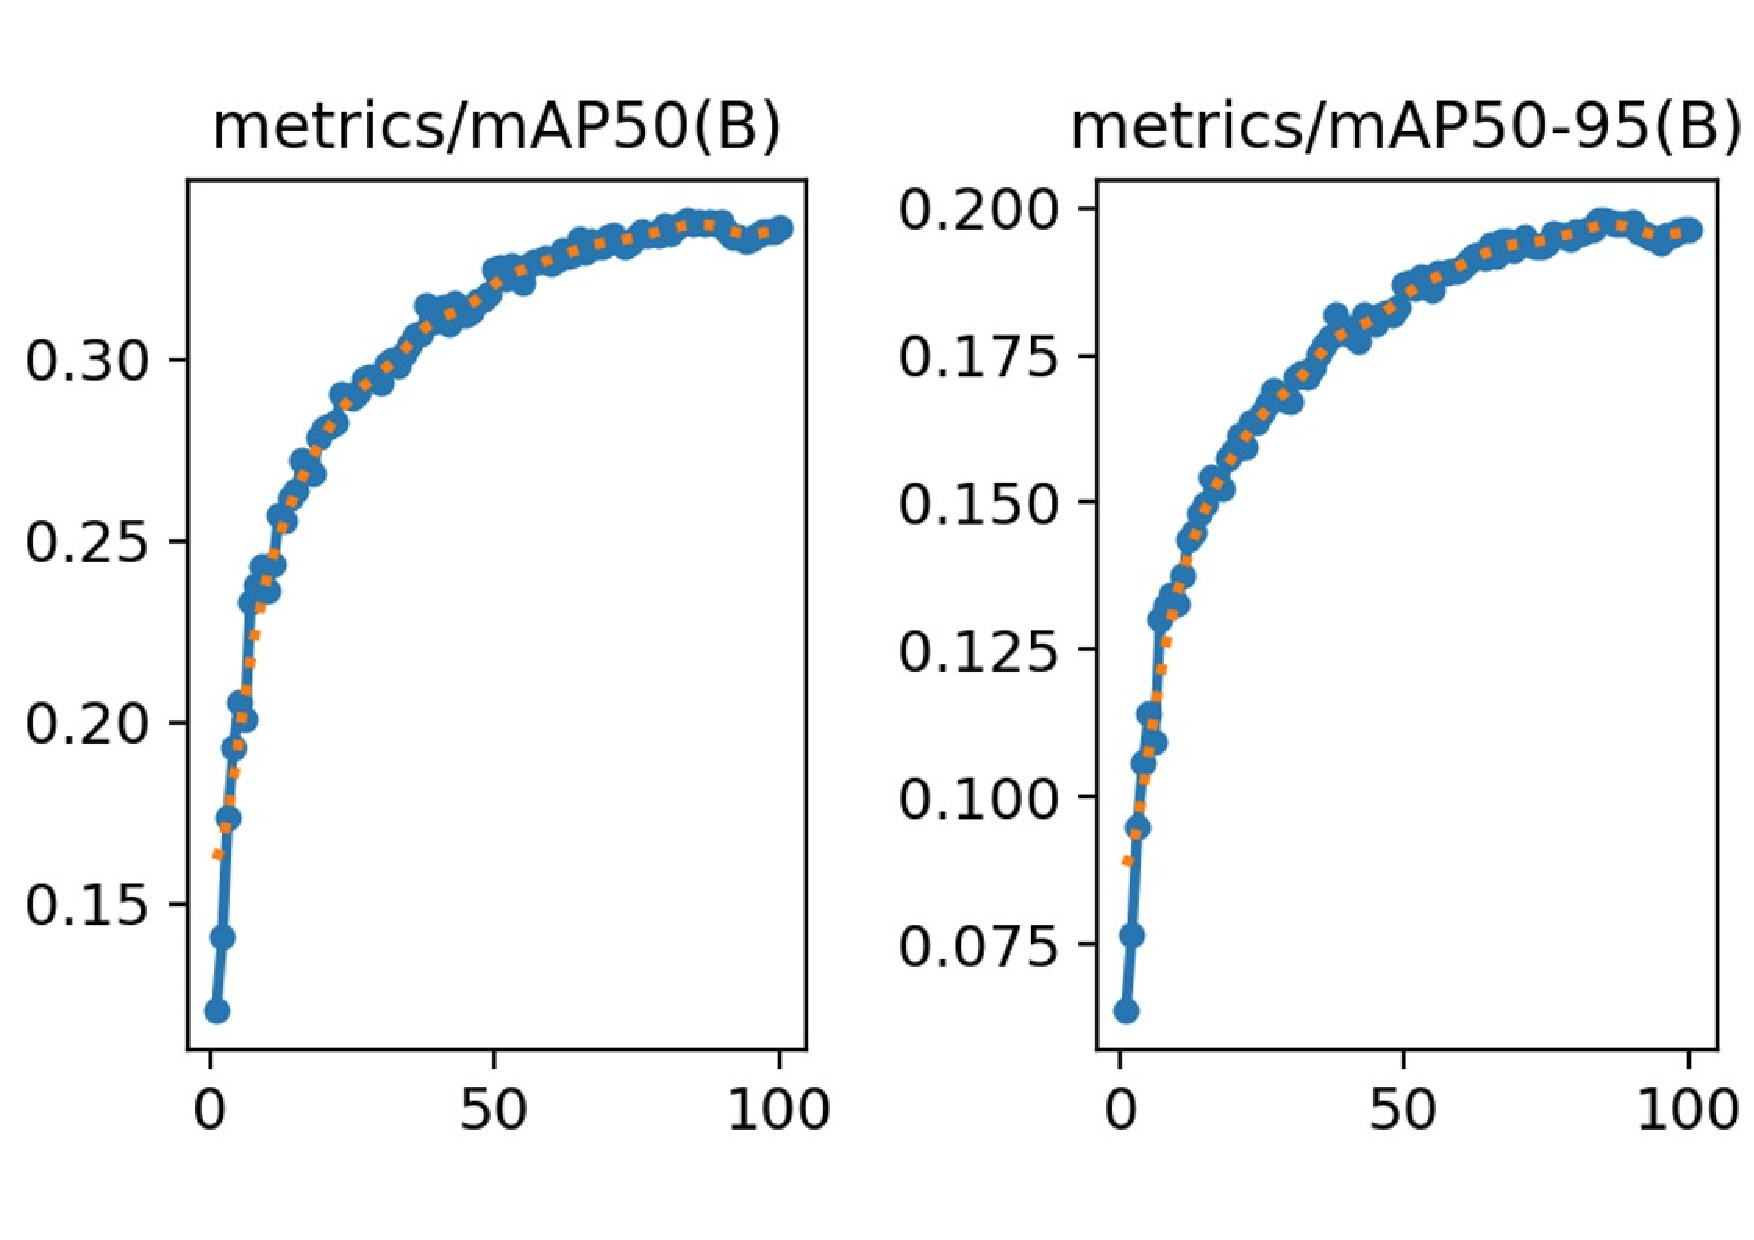
\includegraphics[scale = 0.3]{Cap4/Metrics.pdf}
	\caption{mAP@50 and mAP@50-95 evolution, respectively.}\label{mAPssistema}
\end{figure}

The analysis of those curves shows that the model do not have the best performance. To have a deeper understanding of the problem, a breakdown of mAP for each class is presented in Table \ref{Breakdown mAP}.

\begin{table}[!h]
   \begin{center}
   \caption{mAP@50 and mAP@50-95 for each class.}
   \label{Breakdown mAP}
   \begin{tabular}{|c|c|c|} 
    \hline
    Class & mAP@50 & mAP@50-95 \\ [0.5ex] 
    \hline\hline
    Pedestrian & 0.339 & 0.15 \\ 
    \hline
    People & 0.286 & 0.104 \\
    \hline
    Bicycle & 0.0804 & 0.0328\\
    \hline
    Car & 0.756 & 0.519 \\
    \hline
    Van & 0.384 & 0.266 \\
    \hline
    Truck & 0.301 & 0.202 \\
    \hline
    Tricycle & 0.229 & 0.122 \\
    \hline
    Awning-tricycle & 0.127 &  0.0812\\
    \hline
    Bus & 0.503 & 0.354 \\
    \hline
    Motor & 0.369 & 0.153 \\
    \hline
   \end{tabular}
   \end{center}
   \end{table}

We can see that the class Car has the highest value of mAP, this may occur because the dataset has a large number of images showing cars in different conditions, which will enhance the model's capability of detecting cars. Although that is not the only reason to explain the result, it must be considered. Figure \ref{Instancesperclass} shows the number of instances for each class.
\begin{figure}[H]
	\centering
	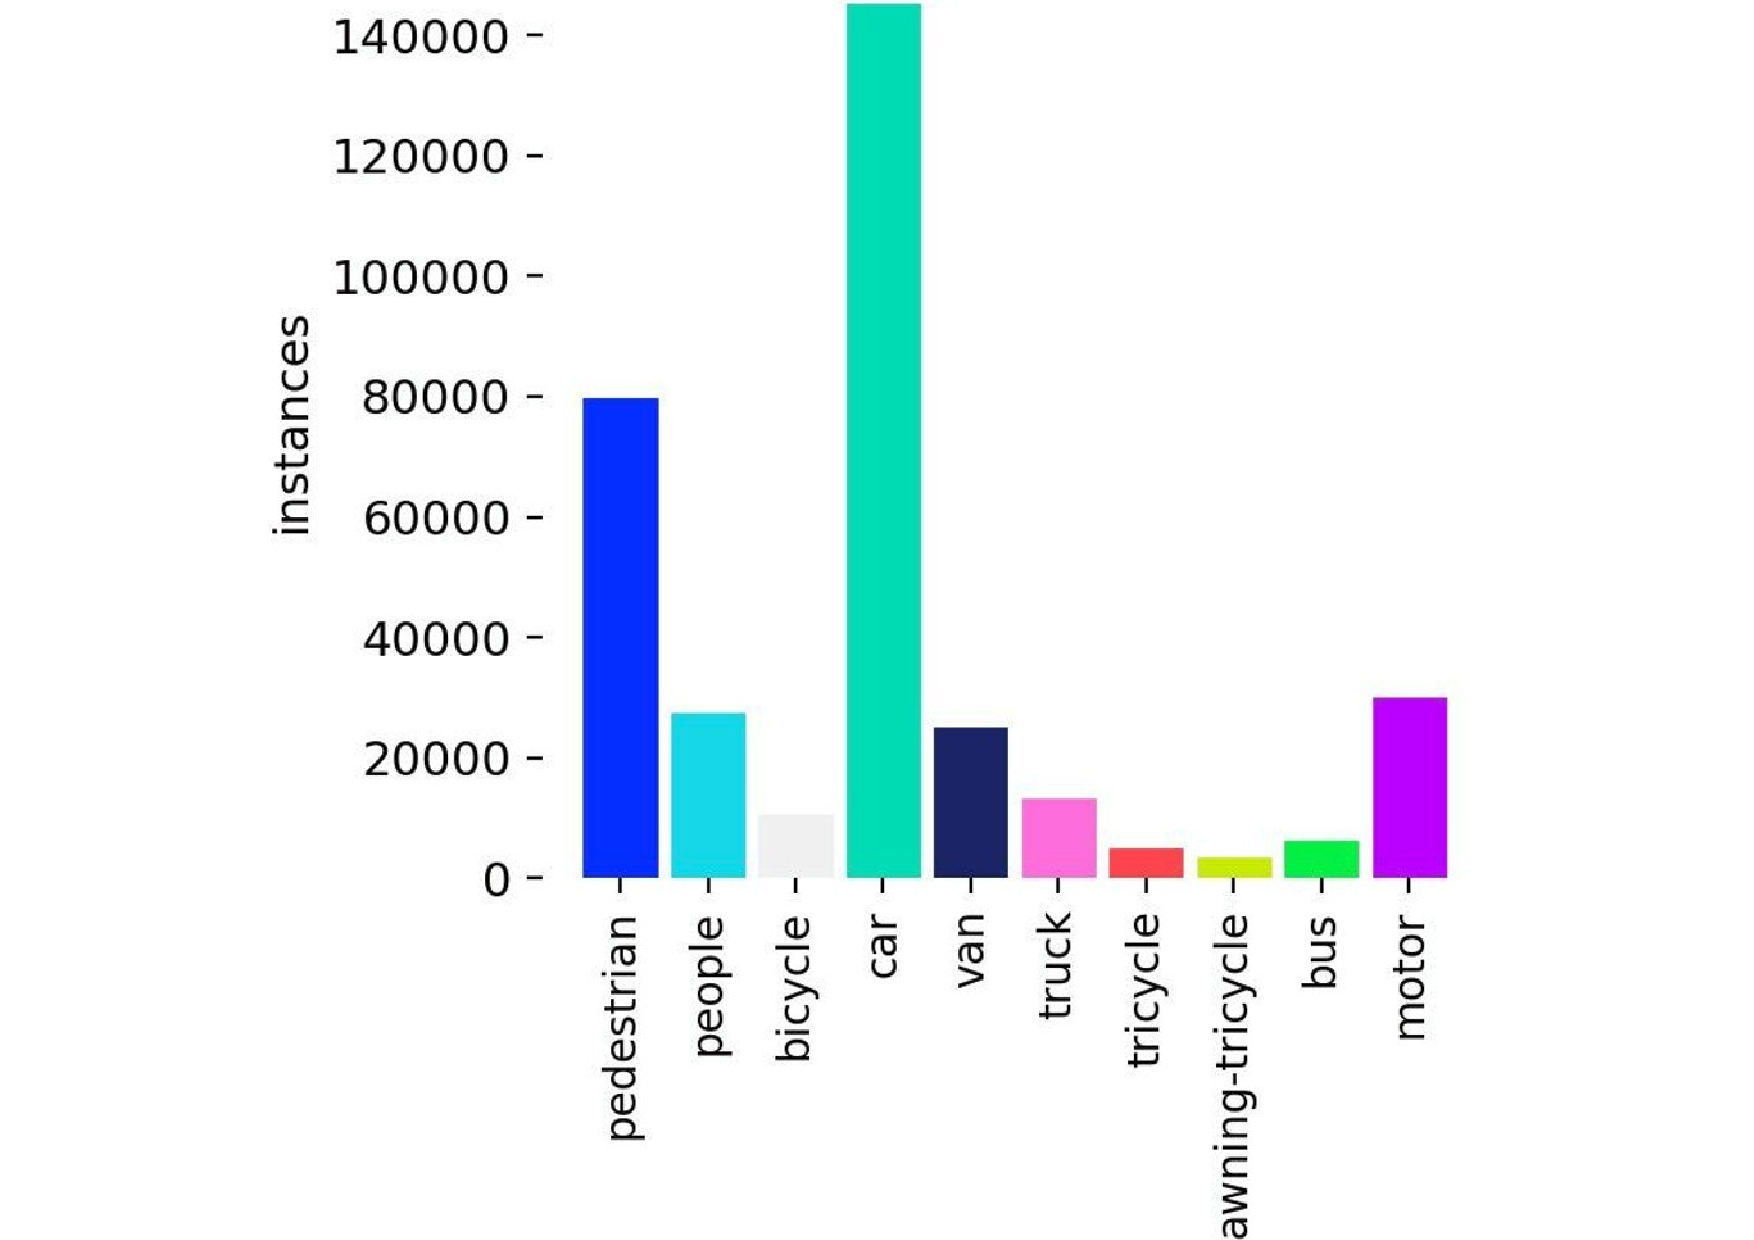
\includegraphics[scale = 0.45]{Cap4/Instances.pdf}
	\caption{Instances per class.}\label{Instancesperclass}
\end{figure}

The results indicate that the dataset is imbalanced. Obaid and Nassif (2022) apply solutions to the dataset imbalance problem by utilizing Resampling approaches, and the results show an increase in the classifier's accuracy. Changing the hyperparameters for training could also enhance the model's performance on object detection tasks.

\section{System Performance}
In this section, we will evaluate the performance of the system with regard to characteristics of the system's response and the communication delay from the implemented UDP protocol.

\subsection{Latency}
In computer data networks, latency is defined as the sum of temporal delays within a network. A delay is caused by the propagation and transmission of data packets within the network. To estimate and evaluate the latency, we will use the methodology proposed by \citen{KIESEL2022238}. The architecture of our network control system is shown in Figure \ref{networksys}, where the communication between the Sensor and Controler is done via UDP, and the communication between controller and actuatuador is considered wired, with an estimated latency of 40 miliseconds, modeled using 2nd order Padé approximation.
\begin{figure}[H]
   \centering
   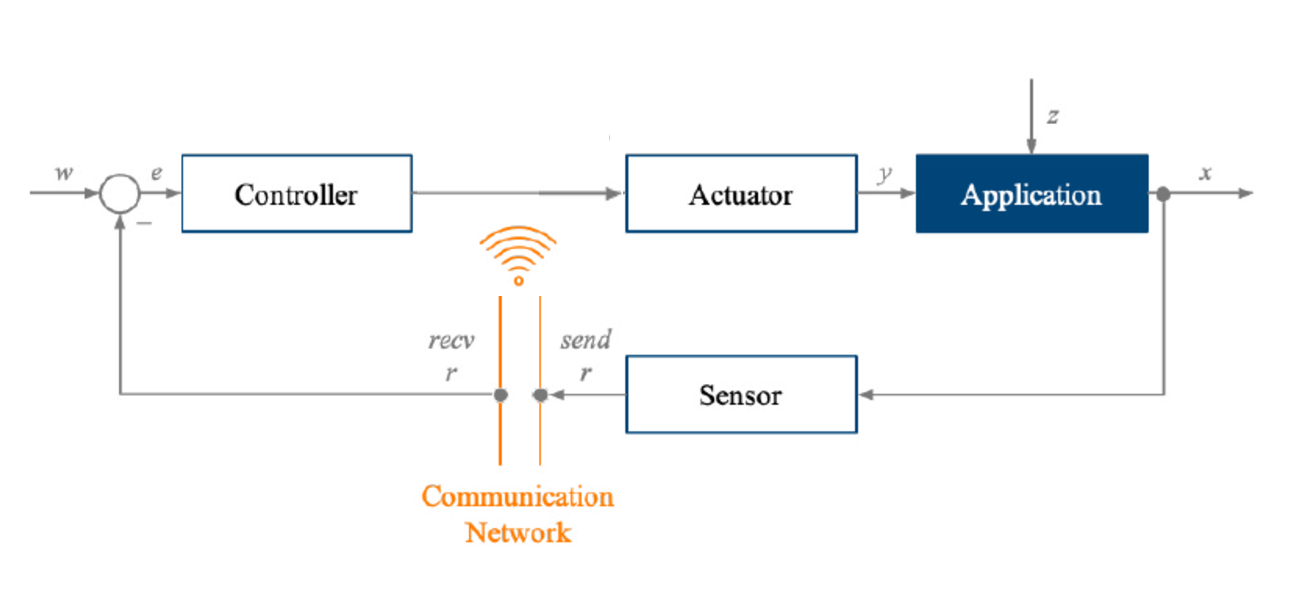
\includegraphics[scale = 0.6]{Cap4/comunication.eps} \\
   \caption{Network communication of the control system. Extracted from \citen{KIESEL2022238}}\label{networksys}
\end{figure}

According to \citen{KIESEL2022238}, the time between event and action, given that each action is triggered by an event, is defined as application-perceived latency. For our system, the application-perceived latency is mathematically expressed as
\begin{equation}
   \Delta \tau_{l,\text{application}} = \tau_{\text{sensor}} + \tau_{\text{controller}} + \tau_{\text{actuator}} + \tau_{\text{network}},
\end{equation}
where $\tau_{\text{sensor}}$ is the time in-between an event is sensed and recorded. $\tau_{\text{controller}}$ expresses the time the controller requires to analyze data from sensor and decide on a control action, which is fed back to the actuator. $\tau_{\text{actuator}}$ describes the time inbetween the reception of the feedback variable and the start of the physical execution of the action. $\tau_{\text{network}}$ describes the time the network requires to transmit data from sensor to controller and from controller to actuator.

To measure $\tau_{\text{sensor}}$ and $\tau_{\text{network}}$, the simulation was changed to generate an object in the image after 10 seconds, then it was observed when the simulation would detect it. Figures \ref{figtest} and \ref{resultgrafic} illustrates the process and the results, respectively.

\begin{figure}[H]
\begin{tabular}{ c c c }
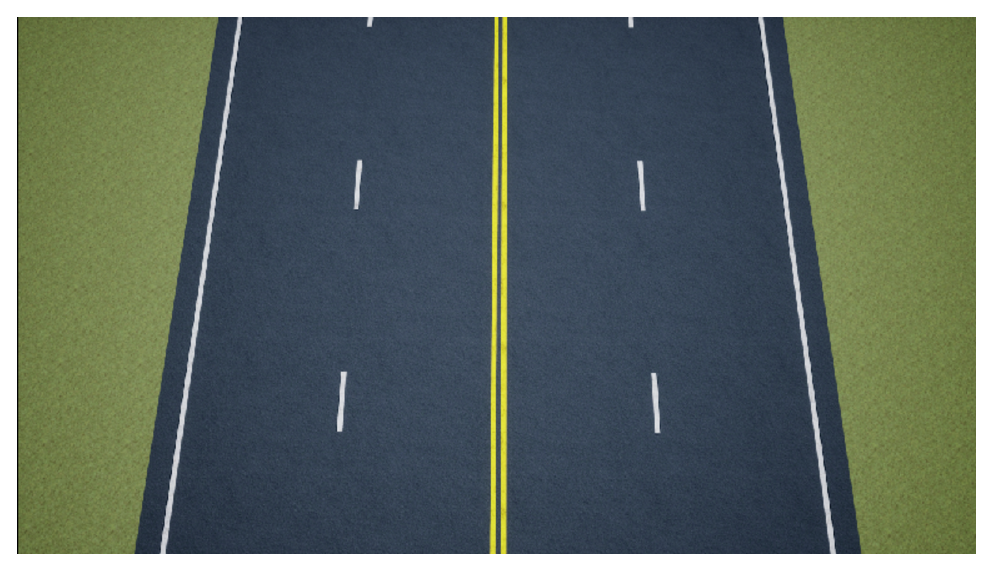
\includegraphics[scale = 0.3]{Cap4/Car3.eps} & 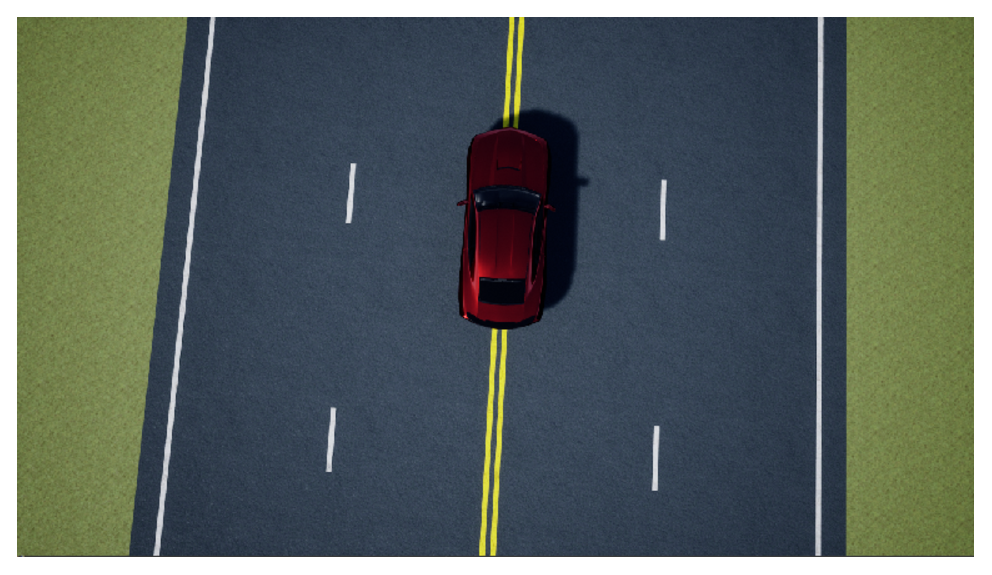
\includegraphics[scale = 0.3]{Cap4/CAR1.eps} & 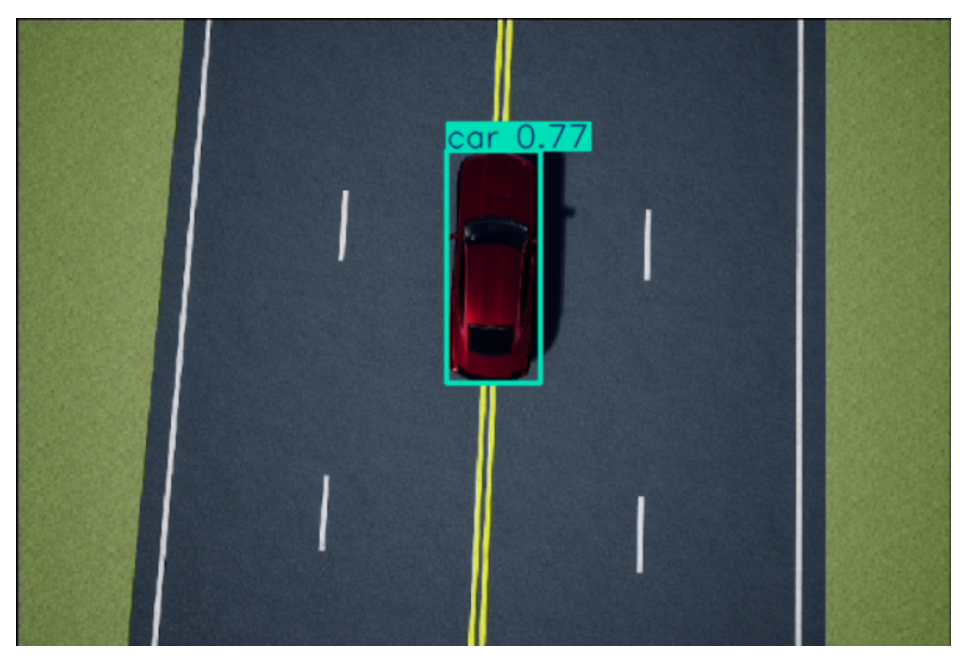
\includegraphics[height=2.8cm]{Cap4/car2.eps} \\
\end{tabular}
\caption{Performed test for latency.}\label{figtest}
\end{figure}

\begin{figure}[H]
   \centering
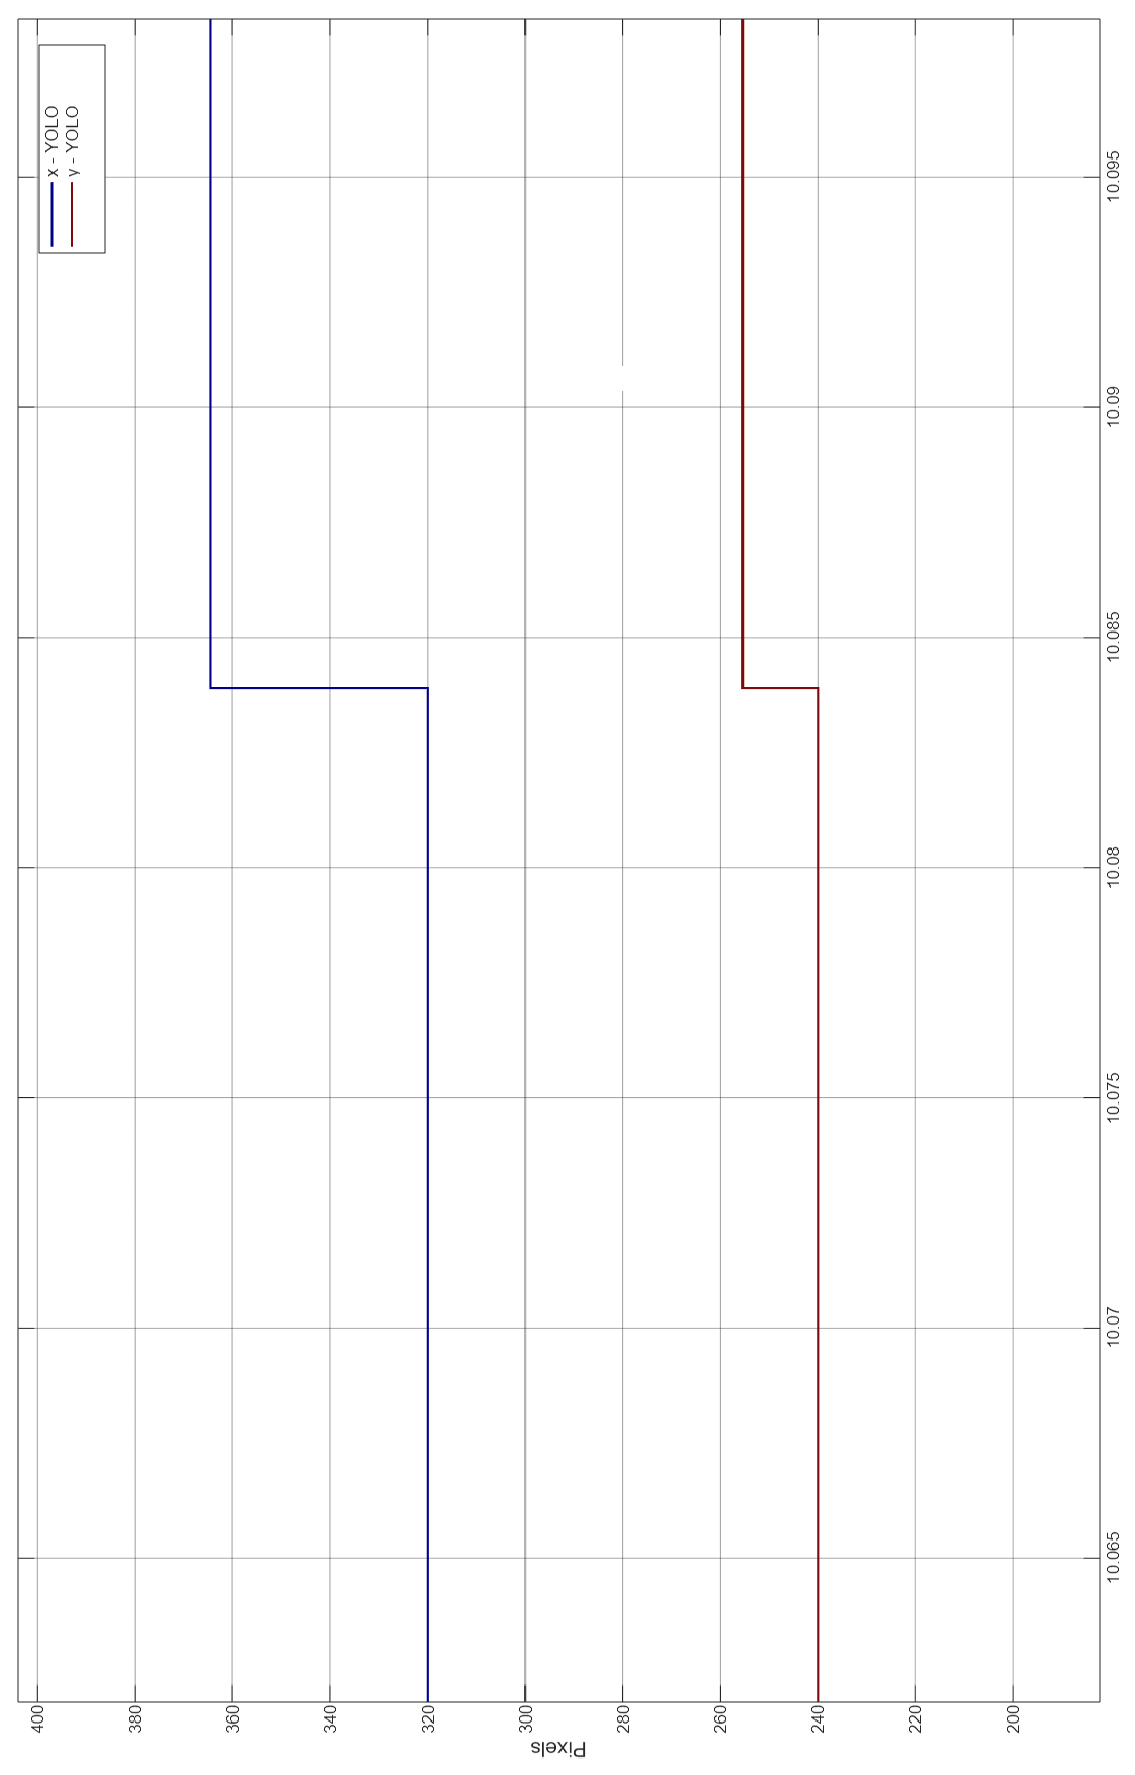
\includegraphics[scale = 0.5, angle = 270]{Cap4/detectedobjpos.eps} \\
\caption{Object recognition delay in seconds.}\label{resultgrafic}
\end{figure}
The results show that the system takes around 84 miliseconds to receive the object's position from the object detection algorithm. This time represents the sum of $\tau_{\text{sensor}}$ and $\tau_{\text{network}}$. Although it is not possible to have a precise measurement of the simulated camera delay, YOLO's processing time is one of the outputs of the object detection algorithm. Since the average time spent by YOLO to process the image is 60 miliseconds, it is estimated that the UDP connection is spending around 24 miliseconds. Thus, $\tau_{\text{sensor}} =$ 60 ms and $\tau_{\text{network}} =$ 24 ms. Given that the Padé approximation is the sum $\tau_{\text{controller}}$ and $\tau_{\text{actuator}}$, the application-perceived latency is approximately
\begin{equation}
   \Delta \tau_{l,\text{application}} = 60 + 40 + 24 = 124 \text{ ms}.
\end{equation}

\subsection{Controlled Output}
To understand how the system is behaving, we generate an input signal representing the angular displacement between the object's position and the principal axis, with reference in 0 (zero), and analyse the system's response. This method allows us to see the system's stability, overshoot and other metrics. Similarly to what was shown in Figure \ref{figtest}, we will create an object in the image after 10 seconds. The test performed and the system's response are shown in Figures \ref{carrotrack} and \ref{Step response elevation}.
\begin{figure}[H]
   \centering
\begin{tabular}{ c  c  c }
   \centering
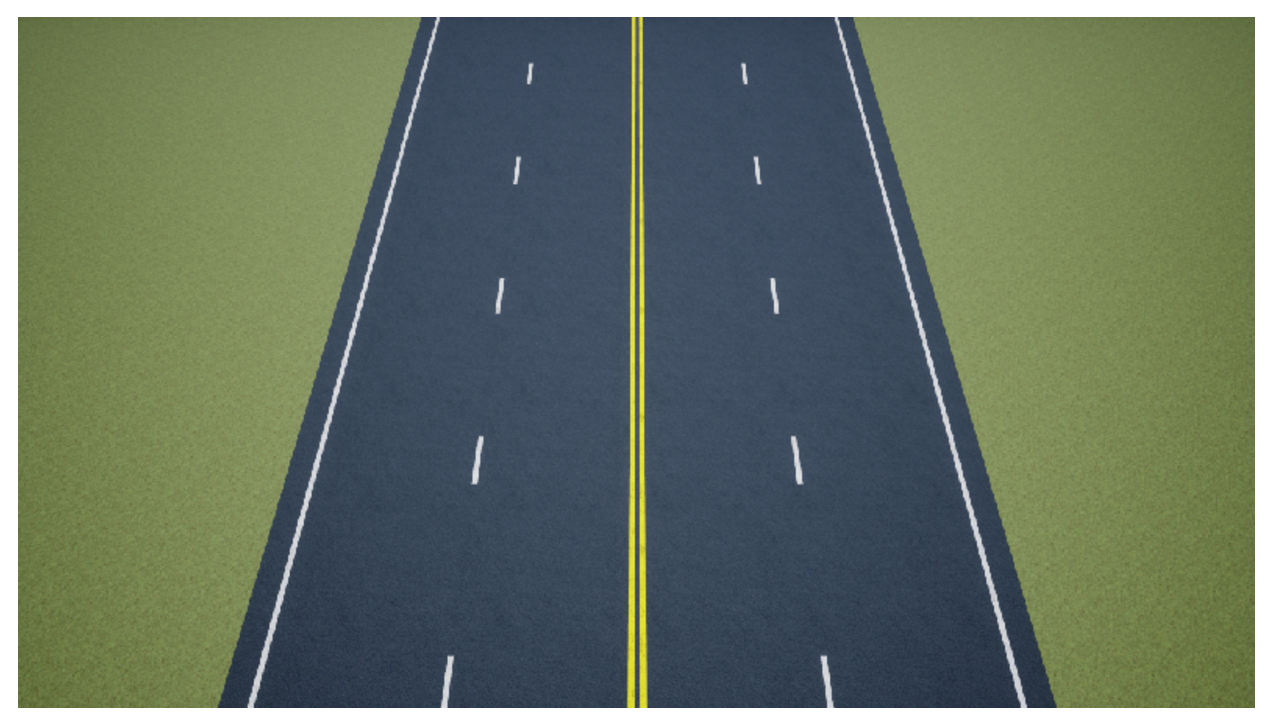
\includegraphics[scale = 0.2]{Cap4/cartracking1.eps} & 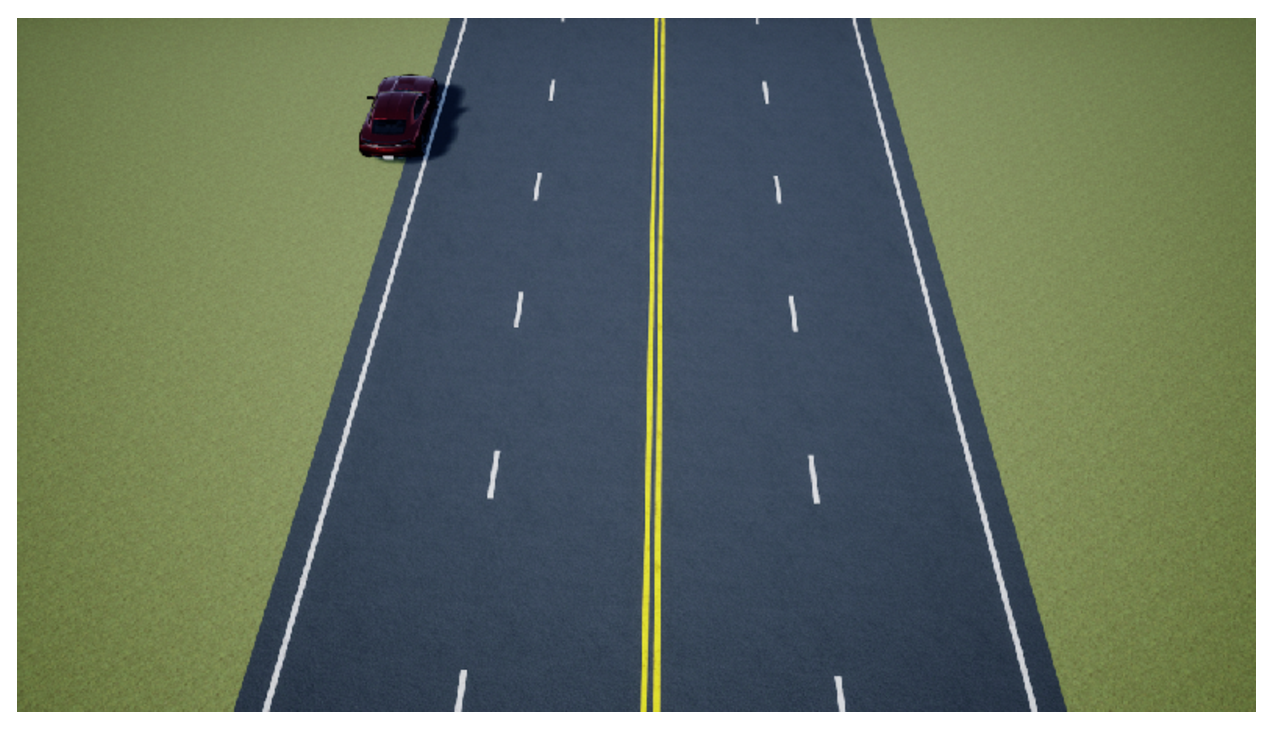
\includegraphics[scale = 0.2]{Cap4/cartracking2.eps} & 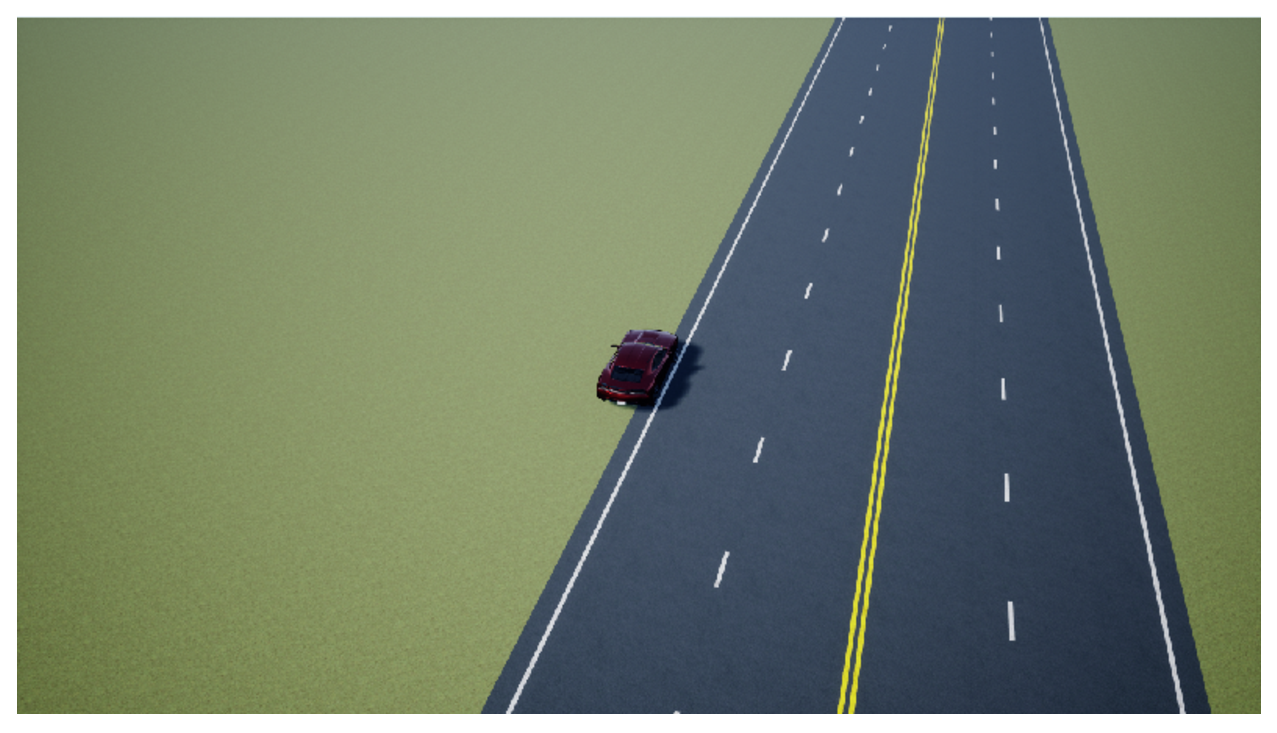
\includegraphics[scale=0.2]{Cap4/cartracking3.eps} \\
\end{tabular}
\caption{Test performed for system behavior analysis.}\label{carrotrack}
\end{figure}

\begin{figure}[H]
	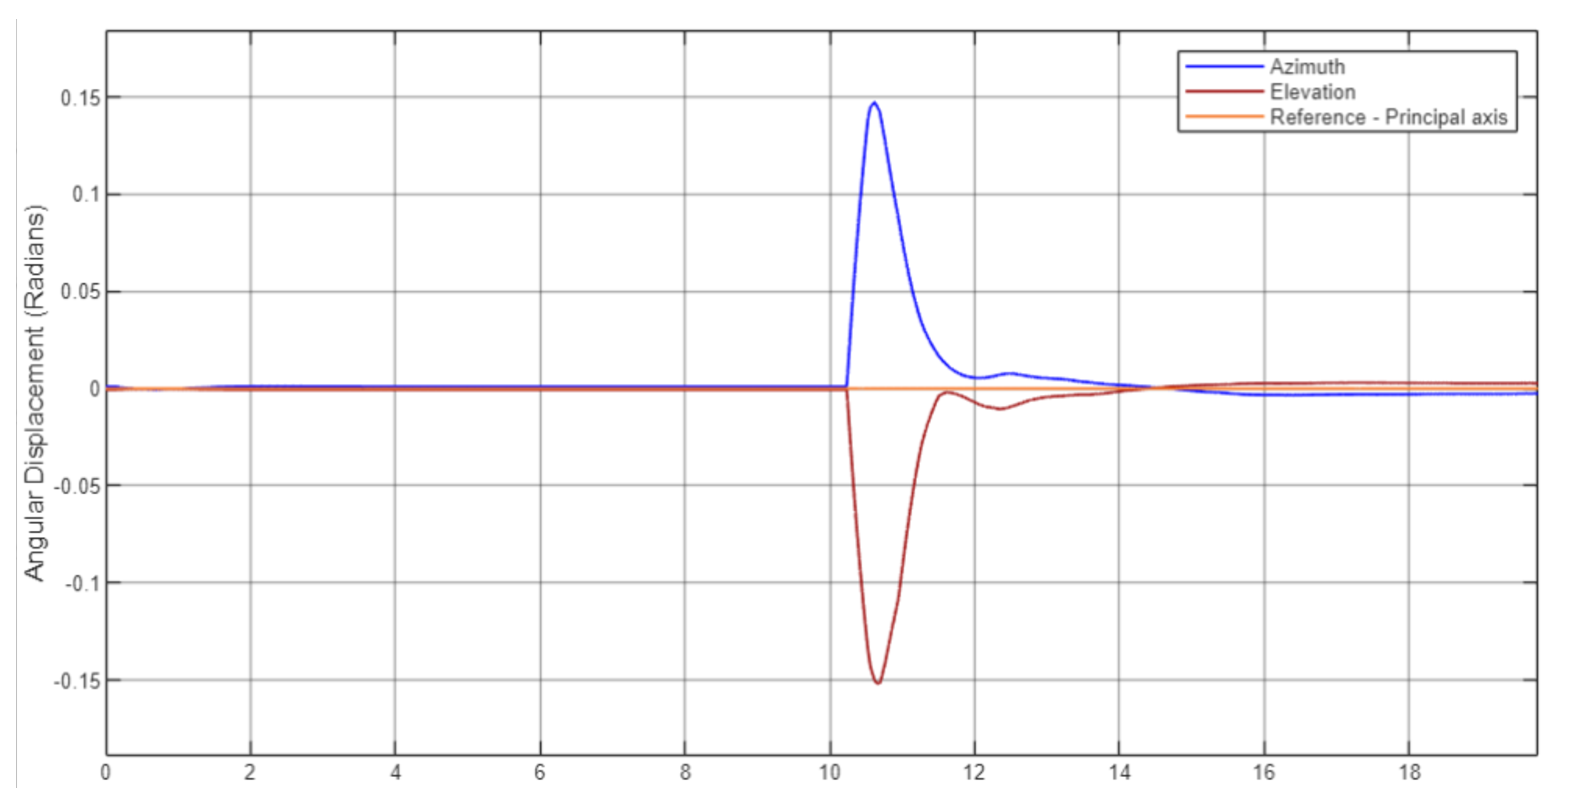
\includegraphics[scale = 0.6]{Cap4/systembehavior.eps}
	\caption{System response to the input signal.}\label{Step response elevation}
\end{figure}
The result shows that the system is stable, although the latency in communication may affect the transient response. In 10 seconds, where the step occurs, it is possible to observe an overshoot for both axes, which leads to an oscilatory behavior that takes around 5 seconds to settle, entering in the steady-state. This shows opportunities for improvement in the system model and the PID controller.
